\documentclass[12pt]{article}

\usepackage{hyperref}
\usepackage[romanian]{babel}
\usepackage{graphicx}
\usepackage[margin=1.25in]{geometry}

\usepackage{lipsum}

\author{Boboi Tomas-Adrian, Cornea Alexandru-Vlad\\ Universitatea Politehnica Timișoara}
\date{Aprilie 2021}
\title{Evaluarea Performanțelor Sistemelor de Calcul\\ Performance Evaluation of Web Services}

\begin{document}
    \maketitle
    \thispagestyle{empty}
    \pagebreak

    \tableofcontents
    \pagenumbering{arabic}
    \pagebreak

    \section{Descrierea sistemului}

        \subsection{Descrierea sistemului din viața reală care se modelează}
            Sistemul modelat în lucrarea aleasă reprezintă o așa-zisă arhitectură orientată pe servicii (Service-oriented Architecture, sau SoA, pe scurt). În cadrul acestei paradigme, serviciile sunt văzute ca entități modulare care pot fi înlănțuite și conectate între ele pentru a obține o funcționalitate nouă, mai complexă decât cea a componentelor individuale care alcătuiesc sistemul.

            Construind un sistem utilizând arhitectura menționată, atât administratorii sistemului, cât și utilizatorii finali se bucură de beneficii pe care un sistem cu o arhitectură cu un grad de modularitate scăzută nu le poate oferi.

            Pe de o parte, costurile de implementare, îmbunătățire ulterioară, dar și de mentenanță suportate de administratorul de sistem sunt mai scăzute, granularitatea sistemului permițând modificări restrânse pe un modul individual sau un set de module bine definit.

            Pe de altă parte, utilizatorii se bucură de un sistem care oferă o per\-for\-man\-ță mulțumitoare, care poate fi ajustată dinamic, in funcție de diverși factori. Acest lucru asigură îndeplinirea țelului utilizatorului cât mai rapid și mai ușor, fapt ce garantează utilizarea viitoare a serviciului de către client.

            \vspace{\baselineskip}
            \noindent
            Sistemul concret din viața reală care se modelează este o agenție de turism care dorește să-și mute activitatea în mediul on-line. Utilizatorii au acces la această aplicație web prin intermediul unei interfețe, numită \textit{Frontend}.

            Utilizatorii aleg mai întâi o locație de pe hartă, după care selectează mijlocul de transport dorit (tren, avion sau taxi).

            Următorul pas este plata, iar utilizatorii care doresc să facă mai multe opriri în călătoriile lor își vor depune călătoria curentă într-un coș de cum\-pă\-ră\-turi. Trebuie menționat aici că aplicația suportă două clase de utilizatori: cei care doresc să planifice o călătorie directă, din punctul A în punctul B, și cei care doresc să-și planifice o călătorie cu opriri intermediare, planificate individual.

            Din cele spuse mai sus, putem deduce serviciile care sunt inlănțuite în cadrul sistemului: \textit{frontend}, \textit{hartă}, \textit{coș de cumpărături}, \textit{tren}, \textit{avion}, \textit{taxi} și \textit{plată}. Imbunătățirea performanței sistemului va presupune imbunătățirea performanțelor serviciilor individuale, fapt ce reprezintă țelul lucrării alese, și al proiectului curent.
            \pagebreak

        \subsection{Descrierea parametrilor care caracterizează sistemul}
            Parametrii care caracterizează sistemul din viața reală sunt timpii de servire ai fiecărui serviciu în parte. Fiecare componentă modulară din sistem are asociat acest timp de servire, care reprezintă timpul scurs între primirea intrării și generarea unei ieșiri spre următorul modul din lanțul sistemului.

            În mod ideal, am dori ca acești timpi să tindă spre zero, însă din considerente de cost și implementare, acest lucru nu este tot timpul posibil. Prețul unui serviciu crește direct proporțional cu calitatea acestuia, astfel încât alegerea în toate cazurile a celor mai performante servicii posibile poate duce la costuri astronomice, care, deși duc la o performanță pe măsură, nu-și justifică costul, clienții neputând sesiza vreo diferență față de un sistem mai ieftin.

            Acesta este unul din scopurile simulării unui asemenea sistem: găsirea combinației de servicii care oferă cea mai bună performanță la prețul cel mai avantajos pentru administratorul de sistem, în funcție de nevoile acestuia și a clienților săi.

            Având în vedere acestea, putem menționa parametrii pe care îi vom folosi pentru a modela și simula sistemul nostru:
            \begin{itemize}
                \item{timpii medii de servire ai fiecărui serviciu}
                    \begin{itemize}
                        \item{servirea se face după o distribuție exponențială, iar acești timpi reprezintă valoarea medie aferentă valorii $\lambda$ care caracterizează distribuția exponențială}
                        \item{timpii de servire corespund fiecărui serviciu în parte, și sunt diferiți în funcție de clasa de utilizatori despre care se discută}
                    \end{itemize}
                \item{probabilitățile de rutare ale serviciului \textit{Frontend}}
                    \begin{itemize}
                        \item{corespondentul lor din viața reală este probabilitatea ca o persoană să acceseze următorul serviciu, pornind de la interfața cu utilizatorul}
                    \end{itemize}
            \end{itemize}
            \pagebreak


    \section{Descrierea modelului construit}

        \subsection{Arhitectura modelului}
            Arhitectura modelului, care poate fi găsită în figura 1, cuprinde serviciile menționate în secțiunea anterioară, modelate ca module de tip \textit{Queue} în contextul programului JMT (Java Modelling Tools). Serviciile sunt următoarele:

            \begin{itemize}
                \itemsep0em
                \item{\textit{Frontend} - interfața cu utilizatorul}
                \item{\textit{Mappe} - serviciul de selectare a unei locații de pe hartă}
                \item{\textit{Carrello} - serviciul care implementează coșul de cumpărături}
                \item{\textit{Aereo}, \textit{Taxi}, \textit{Treno} - serviciile care implementează posibilitatea de a alege între transportul aerian, cu mașina, respectiv cu trenul}
                \item{\textit{Pagamento} - serviciul prin intermediul căruia utilizatorul realizează plata călătoriei, sau a călătoriilor, dacă este un utilizator care alege o călătorie cu mai multe opriri}
            \end{itemize}

            Pe lângă aceste servicii, avem utilizatorii, reprezentați de modului \textit{Utenti}. Aceștia nu mai sunt reprezentați ca un modul de tipul \textit{Queue}, întrucât utilizatorii nu reprezintă un serviciu în sine, ci beneficiarii acestora.

            \begin{figure}[h!]
                \centering
                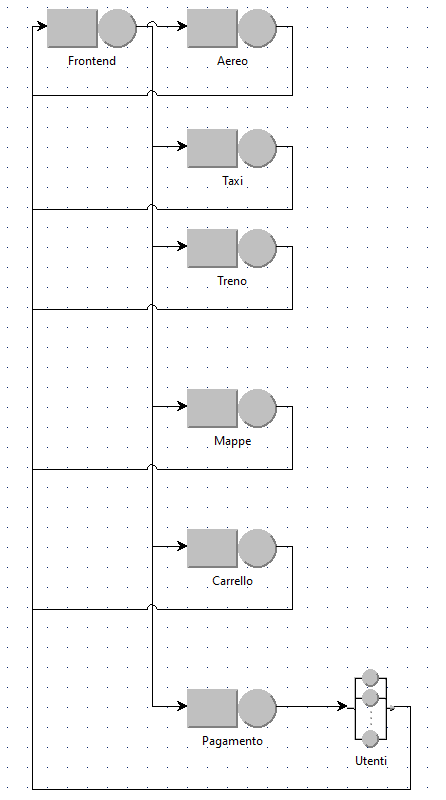
\includegraphics[width=0.45\textwidth]{images/architecture.png}
                \caption{Arhitectura sistemului: utilizatorii accesează diversele servicii oferite de aplicație prin intermediul interfeței cu utilizatorul}
            \end{figure}

        \subsection{Indicii de performanță}
            Indicii de performanță pe care îi studiem în lucrarea curentă sunt următorii:
            \begin{itemize}
                \item{\textit{Utilization} (gradul de utilizare) - reprezintă procentajul din timp în care serviciul este ocupat}
                \item{\textit{System Response Time} (timpul de răspuns al sistemului) - reprezintă timpul de răspuns din punctul de vedere al utilizatorului, mai exact intervalul de timp dintre trimiterea unei cereri din partea utilizatorului și primirea răspunsului}
                \item{\textit{System Throughput} (capacitatea de trecere a sistemului) - reprezintă rata la care utilizatorii realizează o interacțiune completă cu sistemul}
                \item{\textit{Queue Time} (timpul de așteptare) - reprezintă intervalul de timp în care un utilizator așteaptă la nivelul unui centru de servire}
            \end{itemize}

            Indicii aleși sunt folositori pentru a releva performanța sistemului, întucât ei ne oferă atât informații despre calitatea serviciului pentru utilizator, cât și despre performanța sistemului, informații necesare adminsitratorului de sistem.

        \subsection{Valorile inițiale ale indicilor de performanță}
            În figura 2 putem găsi un rezumat al indicilor de performanță. În tabelele următoare se găsesc valorile inițiale ale indicilor de performanță, rezultate în urma procesului de simulare.

            Scopul lucrării studiate este acela de a identifica acele module care îngreunează funcționarea sistemului, prin așa-numitul proces de \textit{bottlenecking}. Identificarea și îmbunătățirea serviciului care produce acest efect va duce la o mai bună performanță a sistemului, iar acesta va fi scopul experimentelor care vor urma în secțiunea 3.
            \pagebreak

            \begin{figure}[!h]
                \centering
                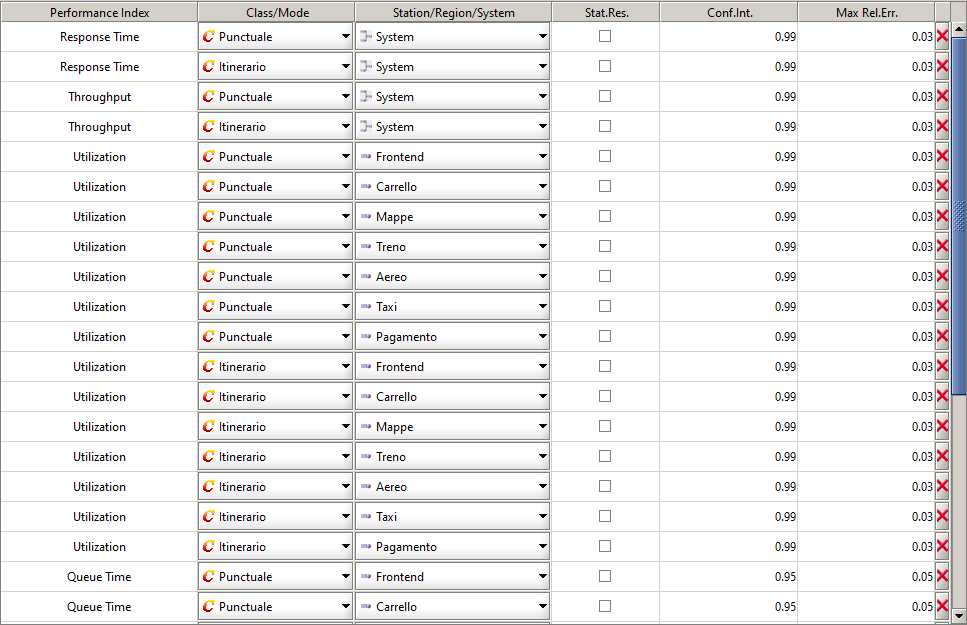
\includegraphics[width=0.85\textwidth]{images/perf_indices.png}
                \caption{Descrierea indicilor de performanță ai sistemului. Din imagine mai lipsesc timpii de așteptare aferenți câtorva module respectiv clase de utilizatori, însă ei se pot regăsi în tabelele de mai jos}
            \end{figure}

            \begin{table}[!h]
                \centering
                \begin{tabular}{r|cclrr|cc}
                    \multicolumn{1}{c|}{Utilization} & "Puntuale" & "Itinerario" &  & \multicolumn{1}{c}{} & \multicolumn{1}{c|}{Queue Time} & "Puntuale"       & "Itinerario"     \\ \cline{1-3} \cline{6-8} 
                    Frontend                         & 0.0120     & 0.1072       &  &                      & Frontend                        & \textbf{5.66E-4} & \textbf{4.98E-4} \\
                    Carello                          & -          & 0.0212       &  &                      & Carello                         & -                & 0.00             \\
                    Mappe                            & 7.44E-3    & 2.55E-3      &  &                      & Mappe                           & 3.18E-6          & 1.41E-5          \\
                    Treno                            & 3.60E-3    & 1.70E-3      &  &                      & Treno                           & 3.80E-6          & 1.48E-5          \\
                    Aereo                            & 2.18E-3    & 1.36E-3      &  &                      & Aereo                           & 2.52E-6          & 4.85E-6          \\
                    Taxi                             & 1.68E-3    & 2.04E-3      &  &                      & Taxi                            & 3.64E-6          & 3.50E-6          \\
                    Pagamento                        & 9.83E-4    & 8.78E-4      &  &                      & Pagamento                       & 1.78E-6          & 1.60E-7         
                \end{tabular}
            \end{table}

            \begin{table}[!h]
                \centering
                \begin{tabular}{r|cc}
                    \multicolumn{1}{c|}{} & "Puntuale" & "Itinerario" \\ \hline
                    System Response Time  & 1.0327     & 1.1548       \\
                    System Throughput     & 0.9683     & 0.8659      
                \end{tabular}
                \caption{Rezultatele inițiale ale simulării. Observăm că serviciul de \textit{Frontend} produce efectul de bottleneck, întrucât timpul de așteptare al său este cel mai pronunțat.}
            \end{table}
            \pagebreak

    \section{Experimente}
        Experimentele ce urmează au ca scop îmbunătățirea performanțelor sistemului, prin identificarea serviciilor care îngreunează sistemul, și înlocuirea lor cu o serie de servicii mai performante. Acesta este avantajul arhitecturilor de tipul Service-oriented, anume că îmbunătățirea sistemului se poate face modular, încă din faza de proiectare, în funcție de necesitățile clienților.

        \subsection{Experimentul \#1}
            În cadrul acestui prim experiment vom îmbunătăți serviciul de \textit{Frontend}, anume îi vom înjumătăți timpul de servire, simulând astfel un serviciu de două ori mai rapid, pentru ambele clase de utilizatori.

            Astfel, noile valori medii (\textit{mean values}) ale timpilor de servire pot fi găsiți în tabelul următor:

            \begin{table}[!h]
                \centering
                \begin{tabular}{r|cc}
                    \multicolumn{1}{c|}{} & "Puntuale"      & "Itinerario"    \\ \hline
                    Frontend              & \textit{0.0010} & \textit{0.0033} \\
                    Carello               &                 & 0.0050          \\
                    Mappe                 & 0.0025          & 0.0005          \\
                    Treno                 & 0.0050          & 0.0010          \\
                    Aereo                 & 0.0030          & 0.0008          \\
                    Taxi                  & 0.0030          & 0.0008          \\
                    Pagamento             & 0.0010          & 0.0010         
                \end{tabular}
                \caption{Valorile medii ale timpilor de servire (urmând o distribuție exponențială) corespunzători serviciilor din sistem. Observăm că pentru clasa \textit{Puntuale}, serviciul \textit{Carello} nu are nicio valoare, fiindcă utilizatorii punctuali nu au posibilitatea de a-și adăuga tichetele în coșul de cumpărături}
            \end{table}

            \begin{figure}[!h]
                \centering
                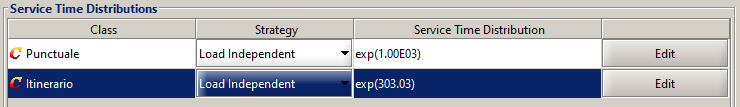
\includegraphics[width=\textwidth]{images/exp1_setup.png}
                \caption{Modificările din JMT făcute în cadrul acestui experiment}
            \end{figure}

            Rezultatele simulării cu noul serviciu de \textit{Frontend} se pot găsi în tabelele de mai jos.
            \pagebreak

            \begin{table}[!h]
                \centering
                \begin{tabular}{r|cclrr|cc}
                    \multicolumn{1}{c|}{Utilization} & "Puntuale" & "Itinerario" &  & \multicolumn{1}{c}{} & \multicolumn{1}{c|}{Queue Time} & "Puntuale"       & "Itinerario"     \\ \cline{1-3} \cline{6-8} 
                    Frontend                         & 6.05E-3    & 0.0570       &  &                      & Frontend                        & \textbf{1.45E-4} & 1.18E-5          \\
                    Carello                          & -          & 0.0229       &  &                      & Carello                         & -                & 0.00             \\
                    Mappe                            & 7.47E-3    & 2.76E-3      &  &                      & Mappe                           & 3.52E-6          & 1.33E-5          \\
                    Treno                            & 3.70E-3    & 1.83E-3      &  &                      & Treno                           & 3.61E-6          & \textbf{1.42E-5} \\
                    Aereo                            & 2.25E-3    & 1.45E-3      &  &                      & Aereo                           & 2.27E-6          & 5.07E-6          \\
                    Taxi                             & 1.73E-3    & 2.19E-3      &  &                      & Taxi                            & 3.37E-6          & 2.80E-6          \\
                    Pagamento                        & 9.92E-4    & 9.27E-4      &  &                      & Pagamento                       & 1.66E-6          & 7.55E-7         
                \end{tabular}
            \end{table}

            \begin{table}[!h]
                \centering
                \begin{tabular}{r|cc}
                    \multicolumn{1}{c|}{} & "Puntuale" & "Itinerario" \\ \hline
                    System Response Time  & 1.0150     & 1.1005       \\
                    System Throughput     & 0.9852     & 0.9087      
                \end{tabular}
                \caption{Rezultatele obținute de pe urma primului experiment}
            \end{table}

            Îmbunătățirea serviciului de \textit{Frontend} duce la o mai bună performanță a sistemului pe toate planurile: gradul de utilizare este mai scăzut, timpul de așteptare a scăzut, timpul de răspuns al sistemului a scăzut și el, iar capacitatea de trecere a sistemului a crescut.

            Deși aceste variații nu par semnificative, trebuie să reținem că simularea s-a realizat cu câte un utilizator în fiecare clasă (la fel ca în lucrarea inițială), \textit{Puntuale}, respectiv \textit{Itinerario}. Scalarea aplicației la un număr mai semnificativ de utilizatori va duce la amplificarea acestor diferențe, și va accentua superioritatea sistemului care conține serviciul de \textit{Frontend} modificat.
        
        \subsection{Experimentul \#2}
            Mai departe, urmărim același scop ca la experimentul precedent, și identificăm acele servicii care produc fenomenul de \textit{bottlenecking}: serviciul \textit{Frontend} pentru clasa de utilizatori \textit{Puntuale}, respectiv serviciul \textit{Treno} pentru clasa de utilizatori \textit{Itinerario}.
            
            Înjumătățim timpii medii de servire aferenți acestor servicii pentru clasele de utilizatori menționate, astfel că, față de valorile din tabela 2, serviciul \textit{Frontend} va avea un timp de servire de 0.0005 unități de timp pentru utilizatorii \textit{Puntuale}, iar serviciul \textit{Treno} va avea un timp de servire de 0.0005 unități de timp pentru utilizatorii \textit{Itinerario}.
            \pagebreak

            \begin{table}[!h]
                \centering
                \begin{tabular}{r|cc}
                    \multicolumn{1}{c|}{} & "Puntuale"      & "Itinerario"    \\ \hline
                    Frontend              & \textit{0.0005} & 0.0033 \\
                    Carello               &                 & 0.0050          \\
                    Mappe                 & 0.0025          & 0.0005          \\
                    Treno                 & 0.0050          & \textit{0.0005} \\
                    Aereo                 & 0.0030          & 0.0008          \\
                    Taxi                  & 0.0030          & 0.0008          \\
                    Pagamento             & 0.0010          & 0.0010         
                \end{tabular}
                \caption{Noile valori ale timpilor de servire}
            \end{table}

            Valorile indicilor de performanță, obținute în urma simulării, se pot găsi în tabelele de mai jos. Observăm că variația performanței sistemului este mult mai mică decât la experimentul precedent, fapt ce ne sugerează că trebuie să începem să căutăm o strategie mai eficientă de îmbunătățire a sistemului.

            \begin{table}[!h]
                \centering
                \begin{tabular}{r|cclrr|cc}
                    \multicolumn{1}{c|}{Utilization} & "Puntuale" & "Itinerario" &  & \multicolumn{1}{c}{} & \multicolumn{1}{c|}{Queue Time} & "Puntuale"       & "Itinerario"     \\ \cline{1-3} \cline{6-8} 
                    Frontend                         & 3.02E-3    & 0.0574       &  &                      & Frontend                        & \textbf{1.40E-4} & 3.92E-6          \\
                    Carello                          & -          & 0.0226       &  &                      & Carello                         & -                & 0.00             \\
                    Mappe                            & 7.56E-3    & 2.74E-3      &  &                      & Mappe                           & 4.90E-6          & 1.26E-5          \\
                    Treno                            & 3.68E-3    & 9.12E-3      &  &                      & Treno                           & 1.54E-6          & \textbf{1.31E-5} \\
                    Aereo                            & 2.22E-3    & 1.46E-3      &  &                      & Aereo                           & 3.08E-6          & 4.74E-6          \\
                    Taxi                             & 1.71E-3    & 2.19E-3      &  &                      & Taxi                            & 4.58E-6          & 5.38E-6          \\
                    Pagamento                        & 9.84E-4    & 9.19E-4      &  &                      & Pagamento                       & 2.25E-6          & 1.06E-6         
                    \end{tabular}
            \end{table}

            \begin{table}[!h]
                \centering
                \begin{tabular}{r|cc}
                    \multicolumn{1}{c|}{} & "Puntuale" & "Itinerario" \\ \hline
                    System Response Time  & 1.0050     & 1.0652       \\
                    System Throughput     & 0.9925     & 0.9211      
                \end{tabular}
                \caption{Rezultatele obținute în urma îmbunătățirii serviciului de \textit{Frontend} pentru utilizatorii \textit{Puntuale}, respectiv a serviciului \textit{Treno} pentru utilizatorii \textit{Itinerario}}
            \end{table}

            Aceste îmbunătățiri, deși minore, ne indică o caracteristică importantă a sistemelor Service-oriented: nu putem înlătura complet fenomenul de \textit{bottlenecking}, întrucât întotdeauna va exista un serviciu care va îngreuna performanța sistemului. Țelul nostru ar trebui să fie mai degrabă găsirea unui compromis între costul fiecărui serviciu în parte și performanța sistemului.
            \pagebreak

    \section{Concluzii}
        În urma experimentelor realizate putem observa câteva caracteristici definitorii pentru sistemele service-oriented.

        În primul rând, observăm că simularea unei astfel de arhitecturi încă din faza de proiectare poate duce la alegerea componentelor optime, care să satisfacă atât nevoile clienților, cât și cele ale administratorului de sistem, oferind un cost optim pentru performanța obținută.

        Modularitatea sistemului permite schimbări localizate, care afectează regiuni izolate din sistem, ceea ce din nou reduce din costurile de îmbunătățire a sistemului după ce acesta este dat înspre folosire publicului.

        Simularea trebuie însă realizată urmând o mentalitate realistă, întrucât îm\-bu\-nă\-tă\-ți\-rea sistemului prin schimbări incrementale ale serviciilor, cum a fost cazul în experimentele prezentate, are un randament care scade odată cu numărul de iterații. Fenomenul poartă denumirea de \textit{diminishing returns}, însemnând că efortul depus pentru îmbunătățirea sistemului duce la variații din ce în ce mai mici.

        Deși fenomenul de \textit{bottlenecking} nu poate fi înlăturat complet, simularea ne permite, atât nouă cât și administratorilor de sistem, să ajungem la un compromis care să mulțumească pe toată lumea. O mică investiție în faza de proiectare poate, astfel, să ducă la beneficii palpabile pe termen lung.

        Viitoare lucrări pe această temă ar trebui să trateze alte strategii de îmbunătățire a sistemului. Printre acestea putem aminti analizarea sectorului demografic pentru care se realizează aplicația, pentru a cunoaște mai bine procentajul din fiecare clasă de utilizatori, și reorganizarea conexiunilor dintre serviciile din sistem pentru a optimiza fluxul de informații.

\end{document}